\documentclass[12pt]{article}
\usepackage{graphicx}
\usepackage{draftwatermark}
\SetWatermarkText{DRAFT}
\SetWatermarkScale{5}

\title{FURST Grating Specification}
\date{Version 0.2.1, 2017-Jun-27}
\author{C.\ Kankelborg}

\begin{document}
\maketitle

\section{Introduction}

The Full-sun Ultraviolet Rocket SpecTrometer (FURST) is a \emph{proposed} NASA sounding rocket mission to obtain well calibrated FUV spectra of the full sun from 120-200\,nm. This document describes the FURST grating. \emph{We are presently requesting a quotation for budgetary purposes, to support the proposal process.}

The spectrometer is a Rowland circle (Abney mount) spectrograph designed for an aberration limited resolution of $\lambda / \Delta\lambda \sim 20,000$. The spectrograph is fed by a convex cylindrical mirror that produces a tall, narrow ($\sim 15\,\mu$m), virtual image of the full sun in lieu of a slit. The feed optic is moved along the Rowland circle to select the wavelength range that falls on the detector. The angles of incidence and diffraction are on the same side of the grating normal, with the shortest wavelengths imaged at near Littrow configuration, to minimize the overall size of the instrument. A Zemax model of the instrument is available upon request.

\section{Grating Description}
Table \ref{tab:spec} lists requirements for the diffraction grating. Dimensions and layout are specified in figure \ref{fig:sketch}. 
The specifications are written around the assumption of a holographic grating, with the aim of minimizing visible stray light (alignment sections will be covered in flight), but we are open to manufacturer recommendations. Visible stray light also drives the roughness requirement. We suspect that the tabulated requirements can be met with a replica grating. If so, replicas may be most economical since we plan to procure two (\S\,\ref{sec:deliverables}).

\begin{figure}
   \begin{center}
      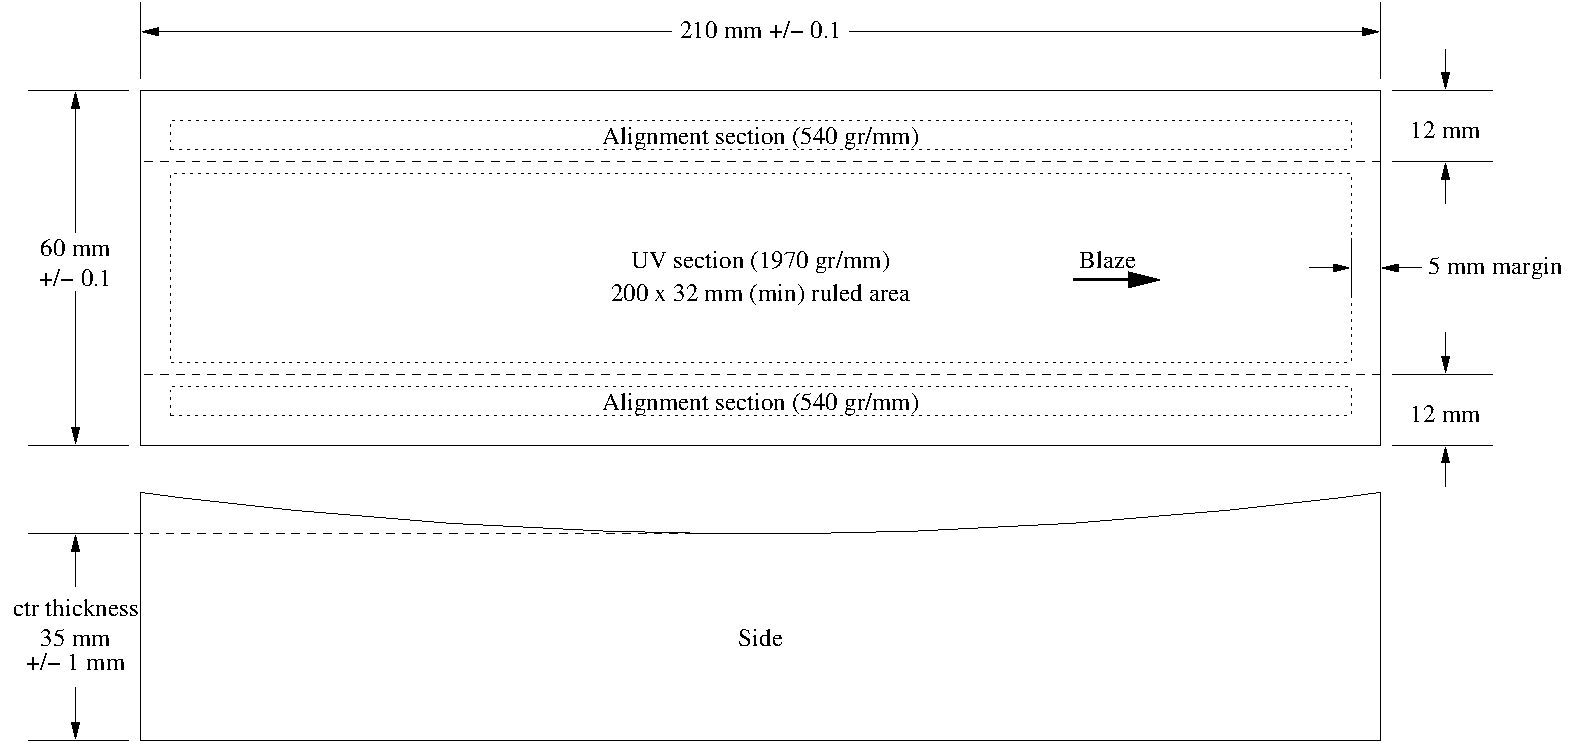
\includegraphics[width=0.99\textwidth]{sketch.pdf}
   \end{center}
   \caption{Sketch of the grating design. Note the two alignment sections, intended for 
      light in the vis-IR, 400-800\,nm.}\label{fig:sketch}
\end{figure}

\begin{table}
\caption{Requirements Table for the FURST grating. Verification methods are T (test), 
   M (measurement), I (inspection), C (calculation), D (design/mfg process).}\label{tab:spec}
   \small
   \begin{tabular}{llc} \hline
      Specification     & Requirement                                     & Verification \\ \hline
      Type              & Concave holographic reflectance grating         & D\\
      Mounting          & Rowland circle (modified Abney)                 & D\\
      Geometry          & Per fig \ref{fig:sketch}                        & I\\
      Figure            & Sphere, $R=1500$\,mm\ $\pm 0.5\%$                 & M\\
      Groove profile    & (quasi-)sinusoidal, optimize for $\lambda 120$\,nm & D\\
      Groove period     & UV and alignment regions per fig \ref{fig:sketch} & D\\
      Spectral order    & $m=1$                                            & D\\
      Groove orientation & UV and alignment regions parallel $\pm 0.2^{\circ}$ & M\\
                        & Grooves perpendicular to long edge $\pm 0.2^{\circ}$ & M\\
      Roughness (along grooves) & $<3.6$\,nm RMS, periods 0.5-50\,$\mu$m  & M\\
      Coating           & Broad band FUV, 120-200\,nm                     & D\\
      UV Section Throughput     & $> 0.2$ \@ $m=1$, $\lambda$120-200\,nm  & C, T\\
      Align Section Throughput & $> 0.2$ \@ $m=1$, $\lambda$400-800\,nm   & C, T\\
      UV Spectral resolution & $\lambda/\Delta\lambda > 20,000$           & C, T\\
      Incidence angle   & $9.10^{\circ} < \alpha < 20.60^{\circ}$           & D\\
      Diffraction angle & $3.51^{\circ} < \beta < 4.69^{\circ}$           & D\\
      Finish            & Fine grind non-optical sides (5)                & I\\
      \hline
   \end{tabular}
   \normalsize
\end{table}
% SURFACE ROUGHNESS RATIONALE
% Note on scattering: Following Jager (2012), the fraction of incident intensity scattered as 'haze' is:
%     H = ( mean(|F(G)|^2) - mean(|F(G)[0,0]|^2) ) ) / mean(|F(G)|^2), 
% where F is the Fourier Transform (or DFT), the means are carried out for wavenumbers smaller (wavelengths larger)
% than the wavenumber (wavelength) of the radiation that is to be scattered, and 
%     G = exp(2ikz[x,y]), where k is the radiation wavenumber and z[x,y] is the surface texture.
% For kz << 1, 
%     G = 1 + 2ikz
% In this limit, and using Parseval's theorem,
%     H = mean( |F(2ikz)|^2 ) / mean(1^2) = 4k^2 mean(z^2) = 16π^2 mean(z^2) / \lambda^2.
% Again with the means taken over wavenumbers smaller than the optical wavenumber. I take the
% roughness to hold over periods longer than ~500 nm, since that's the wavenumber of the dominant solar radiation.
% Looking at SORCE SSI interactively in LISIRD (http://lasp.colorado.edu/lisird/sorce/sorce_ssi/index.html), 
% I get the rough impression that we should suppress visible light by a factor of 1e-5 or better. Suppose
% that our 'solar blind' filter handles the 'or better' part, and require H * Omega/π < 1e-5, where Omega is the
% solid angle of UV grating visible to the detector, and π is the solid angle over which I imagine most of the
% haze will be distributed (less than the unit hemisphere). For our design,
%     Omega = (200/1500) * (32/1500) = 0.004,
% So we want H < π * 1e-5 / Omega  = 0.008, and therefore 
%     mean(z^2) < 0.008 lambda^2/16π^2, or
%     RMS(z) < 0.09 lambda/4π = 
% where the mean is evaluated with periods longer than 500 nm, and for the same reason lambda ~ 500 nm). That's
%     RMS(z) < 3.6 nm, periods > 500 nm = 0.5 µm.
% [Noting limitations of the available objectives and zooms for Zygo profilers, I could derate slightly to 
% periods > 0.55 µm; however, I think this measurement would be trivial for AFM.]
% What's the longest relevant period, the whole optic? That would be difficult!! I think the only relevant
% periods are those capable of scattering 0.5 µm radiation widely. Conservatively, say lambda/period > 0.01 rad. That's
% period < 100 lambda = 50 µm. I think even the highest resolution profiler, on the highest zoom, can sample wider
% than that. It only takes 200 pixels, so that leaves some flexibility on zoom. 
%
% I think I made the above overly complicated. Calculation using Strehl:
% octave:2> (2*pi*0.36/500)^2     % 1 - Strehl
% ans =    2.0466e-05
% octave:3> 1 - 1/exp((2*pi*0.36/500)^2)  % 1 - Strehl, without approximations
% ans =    2.0465e-05
% Apparently, my spec puts H at 2e-5. 

We recognize that throughput and resolution measurements can be challenging in vacuum ultraviolet. Some combination of modeling and testing (the latter perhaps off band) is likely to be necessary. \emph{For purposes of our proposal budget, we request an efficiency estimate supported by calculation.} Verification plan TBD....


\section{Contamination Control}

TBD...minimize both particulate and molecular contamination, consistent with best practice for FUV optics.


\section{Deliverables} \label{sec:deliverables}
\begin{enumerate}
   \item Two coated gratings per specification (flight grating plus spare).
   \item Conformance report for each grating, including all test results relevant to this specification.
\end{enumerate}

\end{document}